\documentclass{article}
\usepackage[margin=1in]{geometry}
\usepackage{url}
\usepackage{booktabs}
\usepackage{forest}
\usepackage{tabu}
\usepackage{listings}
\usepackage{amsmath}
\usepackage{amsfonts}
\usepackage{float}
\usepackage{color}
\usepackage{multicol}
\usepackage[colorlinks = true,
            linkcolor = blue,
            urlcolor  = blue,
            citecolor = blue,
            anchorcolor = blue]{hyperref}
\usepackage{subfig}
\usepackage[font=small,labelfont=bf]{caption} % Required for specifying 
                                              % captions to tables and figures

\newcommand{\MYhref}[3][blue]{\href{#2}{\color{#1}{#3}}}%

\definecolor{dkgreen}{rgb}{0,0.6,0}
\definecolor{gray}{rgb}{0.5,0.5,0.5}
\definecolor{mauve}{rgb}{0.58,0,0.82}

\lstset{frame=tb,
  language=Java,
  aboveskip=3mm,
  belowskip=3mm,
  showstringspaces=false,
  columns=flexible,
  basicstyle={\small\ttfamily},
  numbers=none,
  numberstyle=\tiny\color{gray},
  keywordstyle=\color{blue},
  commentstyle=\color{dkgreen},
  stringstyle=\color{mauve},
  breaklines=true,
  breakatwhitespace=true,
  tabsize=3
}

\title{CPSC 524 Assignment 3: Parallel Matrix Multiplication}
\author{Rami Pellumbi\thanks{M.S., Statistics \& Data Science}}
\date{\today}

\begin{document}

\maketitle

\newpage 

\section{Introduction}

This assignment investigates the implementation and performance of an MPI-
based program tasked with parallel computation of large double precision matrices.
The program's objective is to effectively utilize multiple processors to perform 
the multiplication, optimizing the use of system resources and minimizing 
computation time. The implementation required careful consideration of data 
distribution and process synchronization, ensuring accuracy while maximizing 
computational efficiency. Performance analysis focuses on the scalability of the solution across various 
matrix sizes and the number of processors used. This report outlines the design 
considerations, describes the implementation strategy, and presents an 
evaluation of the program's computational performance.

\section{Project Organization}

The project is laid out as follows:

\begin{multicols}{2}
    \begin{forest}
        for tree={
            font=\ttfamily,
            grow'=0,
            child anchor=west,
            parent anchor=south,
            anchor=west,
            calign=first,
            edge path={
                \noexpand\path [draw, \forestoption{edge}]
                (!u.south west) +(7.5pt,0) |- node[fill,inner sep=1.25pt] {} (.child anchor)\forestoption{edge label};
            },
            before typesetting nodes={
                if n=1
                {insert before={[,phantom]}}
                {}
            },
            fit=band,
            before computing xy={l=15pt},
        }
    [
        [docs/]
        [part1
            [Makefile]
            [runtask1.sh]
            [runtask2.sh]
            [runtask3.sh]
            [task1.c]
            [task2.c]
            [task3.c]
        ]
        [part2
            [bin/]
            [include/]
            [out/]
            [src/]
            [build-run-mpi.sh]
            [build-run-serial.sh]
            [build-run-task5.sh]
            [build-run-task6.sh]
            [build-run-task7.sh]
            [build-run-task8.sh]
            [Makefile]
        ]
    ]
    \end{forest}
    \columnbreak
    \begin{itemize}
        \item \textbf{docs/}: This folder contains LaTeX files and other documentation materials that pertain to the report.
        \item \textbf{part1/}: Code for MPI basics and part 1 tasks.
        \item \textbf{part2/}: Code for parallel matrix multiplication.
        \begin{itemize}
            \item \textbf{bin/}: The \texttt{bin} folder holds compiled objects and executable files, centralizing the output of the compilation process.
            \item \textbf{include/}: Here, all the header files (\texttt{.h}) are stored. 
            \item \textbf{out/}: The \texttt{out} folder stores the outputs from each task. It also houses the csv file containing data generated by the programs.
            \item \textbf{src/}: This directory houses the source files (\texttt{.c}) that make up the benchmarks.
            \item \textbf{Shell Scripts}: The shell scripts are used to submit the job for the relevant task to slurm via \texttt{sbatch}.  
        \end{itemize}
    \end{itemize}
\end{multicols}

\section{Code Explanation, Compilation, and Execution}

This section outlines the steps required to build and execute the code. The provided Bash scripts automate the entire process, 
making it straightforward to compile and run the code. All the below steps assume 
you are in the root of the project directory.

\subsection{Automated Building and Execution}
\begin{itemize}
    \item \textbf{Part 1: Understanding MPI Basics} 
    All part 1 related code is in the \texttt{part1/} directory.
    There are three scripts for part 1, one for each task
    The commands \texttt{sbatch runtask1.sh}, \texttt{sbatch runtask2.sh}, 
    and \texttt{sbatch runtask3.sh} will compile and run the files 
    \texttt{task1.c}, \texttt{task2.c}, and \texttt{task3.c}, respectively.
    
    \item \textbf{Part 2: Parallel Matrix Multiplication}
    All part 2 related code is in the \texttt{part2/} directory.
    There are multiple programs run in Part 2: 
    \begin{itemize}
        \item \texttt{serial.c} Simple, serial, matrix multiplication. Use \texttt{build-run-serial.sh} script to run.
        \item \texttt{task5.c}: Parallel matrix multiplication of square matrices with blocking collectives. 
        Assumes that the number of rows is evenly divisible by the number of processes.
        \item \texttt{task6.c}: Parallel matrix multiplication of square matrices with non blocking collectives. 
        Assumes that the number of rows is evenly divisible by the number of processes.
        \item \texttt{task7.c}:  Parallel matrix multiplication of square matrices with non blocking collectives, 
        with a focus on interleaving communication and computation. Assumes that the number of rows is evenly divisible by the number of processes.
        \item \texttt{taks8.c} Parallel matrix multiplication of square matrices with blocking collectives. 
        Appropriately handles when the number of rows is not evenly divisible by the number of processes.
    \end{itemize}
    To run all the MPI experiments, execute \texttt{sbatch build-run-mpi.sh} from the \texttt{part2} directory. Additionally, 
    each task has its own individual run script: \texttt{build-run-taskX.c}, where \texttt{X} is one of $5,6,7$, or $8$.
    The results will be stored in \texttt{part2/out/results.csv}.
\end{itemize}

\subsection{Post-Build Objects and Executables}
For part 2, upon successful compilation and linking, an \texttt{obj/} subdirectory will be generated within the directory. 
This directory will contain the compiled output files. Additionally, the executable files for running each part will be 
situated in the \texttt{bin/} subdirectory.

\subsection{Output Files From \texttt{sbatch}}
For part 1, the output files generated from running the code by submitting the relevant Bash script via \texttt{sbatch} will be 
in the \texttt{part1} directory. 
For part 2, the output files generated from running the code by submitting the relevant Bash script via \texttt{sbatch} will be 
stored in the \texttt{out} directory. 

\section{MPI Basics}
\subsection{Task 1: Basic Communication Between Processes}
In task 1, we simply run the provided \texttt{task1.c} code. We observe that 
the print statements and appear in first-come-first-served order.
\begin{verbatim}
    Node List:
    r918u05n[01-02]
    ntasks-per-node =  2
    
    Run 1
    Message printed by manager: Total elapsed time is 0.005460 seconds.
    From process 2: I worked for 5 seconds after receiving the following message:
        Hello, from process 0.
    From process 3: I worked for 10 seconds after receiving the following message:
        Hello, from process 0.
    From process 1: I worked for 15 seconds after receiving the following message:
        Hello, from process 0.
    real	0m15.668s
    user	0m0.143s
    sys	0m0.316s
    
    Run 2
    Message printed by manager: Total elapsed time is 0.006188 seconds.
    From process 2: I worked for 5 seconds after receiving the following message:
        Hello, from process 0.
    From process 3: I worked for 10 seconds after receiving the following message:
        Hello, from process 0.
    From process 1: I worked for 15 seconds after receiving the following message:
        Hello, from process 0.
    real	0m15.779s
    user	0m0.146s
    sys	0m0.318s
    
    Run 3
    Message printed by manager: Total elapsed time is 0.007760 seconds.
    From process 2: I worked for 5 seconds after receiving the following message:
        Hello, from process 0.
    From process 3: I worked for 10 seconds after receiving the following message:
        Hello, from process 0.
    From process 1: I worked for 15 seconds after receiving the following message:
        Hello, from process 0.
    real	0m15.614s
    user	0m0.142s
    sys	0m0.301s
\end{verbatim}

\subsection{Task 2: Handling Prints in the Manager}
Here, we modify the provided \texttt{task1.c} remove prints from the non-manager 
processes and instead have the manager print out the messages in rank order. To 
handle this, each worker now sends its message back to the manager:
\begin{lstlisting}
    sprintf(message, "Hello manager, from process %d after working %d seconds.",
             rank, worktime);
    /* Send message back to manager */
    MPI_Send(message, strlen(message) + 1, MPI_CHAR, 0, type, MPI_COMM_WORLD);
\end{lstlisting}
which waits for them like so
\begin{lstlisting}
    /* Receive messages from the workers */
    for (size_t i = 1; i < size; i++)
    {
        MPI_Recv(message, 100, MPI_CHAR, i, type, MPI_COMM_WORLD, &status);
        sleep(3);
        printf("Message from process %d: %s\n", i, message);
    }
\end{lstlisting}
The print out of this program correctly shows the messages printing out in rank order:
\begin{verbatim}
    Node List:
    r918u05n[01-02]
    ntasks-per-node =  2

    Run 1
    Message from process 1: Hello manager, from process 1 after working 15 seconds.
    Message from process 2: Hello manager, from process 2 after working 5 seconds.
    Message from process 3: Hello manager, from process 3 after working 10 seconds.
    Message printed by manager: Total elapsed time is 24.021217 seconds.
    real	0m24.974s
    user	0m15.186s
    sys	0m0.231s
    
    Run 2
    Message from process 1: Hello manager, from process 1 after working 5 seconds.
    Message from process 2: Hello manager, from process 2 after working 10 seconds.
    Message from process 3: Hello manager, from process 3 after working 15 seconds.
    Message printed by manager: Total elapsed time is 18.012530 seconds.
    real	0m18.572s
    user	0m9.184s
    sys	0m0.281s
    
    Run 3
    Message from process 1: Hello manager, from process 1 after working 15 seconds.
    Message from process 2: Hello manager, from process 2 after working 10 seconds.
    Message from process 3: Hello manager, from process 3 after working 5 seconds.
    Message printed by manager: Total elapsed time is 24.000228 seconds.
    real	0m24.574s
    user	0m15.176s
    sys	0m0.219s
\end{verbatim}

\subsection{Task 3: Consistent Performance}
In \texttt{task2.c}, we observe a different elapsed time based on the work 
done by each process. Since the receive is waiting on the ranks in rank order, 
there are scenarios where there is not an efficient overlap between simulated work and 
communication. To remedy this, the manager's receive is changed to any source 
and the messages are stored in a new array of messages instantiated by the manager. 
We use the \texttt{status.MPI\_SOURCE} from the status of the receive to appropriately 
place into the array. Concretely, the manager now does the following.
\begin{lstlisting}
    if (rank == 0)
    {
        char **messages = (char **)malloc((size - 1) * sizeof(char *));
        for (int i = 0; i < size - 1; ++i)
        {
            messages[i] = (char *)malloc(100 * sizeof(char));
        }

        sparm = rwork(0, 0); // initialize the workers' work times

        /* Create the message using sprintf */
        sprintf(message, "Hello, from process %d.", rank);

        MPI_Barrier(MPI_COMM_WORLD);
        wct0 = MPI_Wtime();

        /* Send the message to all the workers, which is where the work happens */
        for (i = 1; i < size; i++)
        {
            MPI_Send(message, strlen(message) + 1, MPI_CHAR, i, type, MPI_COMM_WORLD);
            MPI_Send(&sparm, 1, MPI_INT, i, type, MPI_COMM_WORLD);
        }

        // Receive messages from workers as they complete
        for (int i = 1; i < size; i++)
        {
            MPI_Recv(message, 100, MPI_CHAR, MPI_ANY_SOURCE, type, MPI_COMM_WORLD, &status);
            sleep(3); // Simulate post processing
            strcpy(messages[status.MPI_SOURCE - 1], message);
        }

        /* print messages */
        for (size_t i = 1; i < size; i++)
        {
            printf("Message from process %d: %s\n", i, messages[i - 1]);
        }

        wct1 = MPI_Wtime();
        // timing(&wct1, &cput); // get the end time using the original timing routine
        total_time = wct1 - wct0;
        printf("Message printed by manager: Total elapsed time is %f seconds.\n", total_time);

        for (int i = 0; i < size - 1; i++)
        {
            free(messages[i]);
        }
        free(messages);
    }
\end{lstlisting}
The printout from this execution observed consistent, optimal runtime:
\begin{verbatim}
    Node List:
    r918u05n[01-02]
    ntasks-per-node =  2
    
    Run 1
    Message from process 1: Hello manager, from process 1 after working 15 seconds.
    Message from process 2: Hello manager, from process 2 after working 5 seconds.
    Message from process 3: Hello manager, from process 3 after working 10 seconds.
    Message printed by manager: Total elapsed time is 18.001310 seconds.
    real	0m18.730s
    user	0m9.118s
    sys	0m0.201s
    
    Run 2
    Message from process 1: Hello manager, from process 1 after working 5 seconds.
    Message from process 2: Hello manager, from process 2 after working 15 seconds.
    Message from process 3: Hello manager, from process 3 after working 10 seconds.
    Message printed by manager: Total elapsed time is 18.000172 seconds.
    real	0m18.589s
    user	0m9.130s
    sys	0m0.300s
    
    Run 3
    Message from process 1: Hello manager, from process 1 after working 10 seconds.
    Message from process 2: Hello manager, from process 2 after working 5 seconds.
    Message from process 3: Hello manager, from process 3 after working 15 seconds.
    Message printed by manager: Total elapsed time is 18.000061 seconds.
    real	0m18.584s
    user	0m9.107s
    sys	0m0.267s
\end{verbatim}
It is evident that the post processing time is better overlapped with the communication by communicating 
in this way, thus leading to a faster runtime.

\section{Parallel Matrix Multiplication}
At a high level, we have input $N \times N$ matrices $A$ and $B$, and an output $N \times N$ matrix $C$..
The input matrices, \(A\) and \(B\), are divided into blocks of rows and columns, respectively. 
Each block row of matrix \(A\) is then multiplied with the corresponding block column of matrix \(B\) 
to compute a segment of the resultant matrix \(C\). This block-wise computation enables the distribution 
of the workload among the available processors in the MPI environment. The distribution and collection of data blocks 
utilize MPI's collective communication operations, ensuring that each processor has the necessary data to perform 
its assigned calculations. The final step involves aggregating the computed blocks from all processors to form the complete resultant matrix.
The implementation of the parallel matrix multiplication algorithm follows the ring-pass strategy, which is outlined as follows for the case where $N$ is divisible by $p$ (the number of processes):
\begin{enumerate}
    \item The manager initializes memory of $A$, $B$, and $C$ and initializes $A$ and $B$ with the data to be multiplied.
    \item The manager partitions $A$ and $C$ into $p$ blocks rows each. It partitions $B$ into $p$ block columns.
    \begin{itemize}
        \item $A$ and $C$ are of dimension $(N/p) \times N$.
        \item $B$ is of dimension $N \times (N/p)$.
    \end{itemize}
    \item The manager permanently assigns to each MPI process one block row each of $A$ and $C$, and it assigns 
    each MPI process one block column of $B$ as its initial assignment.
    \item The computation proceeds iteratively until completed:
    \begin{enumerate}
        \item Each MPI process does all the computation it can with the data at hand.
        \item MPI processes then pass their block columns of $B$ to the next higher-ranked MPI process.
    \end{enumerate}
    \item The manager uses MPI collective operations to assemble the full $C$ matrix by collecting 
    all block rows of $C$ from the other MPI processes.
\end{enumerate}

\subsection*{Task 5: Blocking Collectives}
The first attempt at this algorithm was utilizing MPI's blocking collectives. Namely, 
\begin{enumerate}
    \item The manager process initializes matrices $A$ and $B$ with random double
    precision values and creates an empty matrix $C$ to store the result.
    \item \texttt{MPI\_Scatter} is used to distribute the blockes of $A$, $B$, and $C$ across all processes.
    \item Each process computes a partial result by multiplying its block of A with the corresponding block of B and stores it in the appropriate sub-block of \texttt{blockC}.
    \item The partial results are stored in the local block of matrix C, \texttt{blockC}.
    \item Processes then pass their block of $B$ to the next process using \texttt{MPI\_Send} and \texttt{MPI\_Recv}.
    \begin{itemize}
        \item To avoid deadlock, even-ranked processes send before they receive and odd-ranked processes receive before they send.
        \item Each process makes use of a secondary \texttt{blockB} buffer, named \texttt{tempB}, else a process may overwrite its initial segment of $B$ before it is able to use it in a matrix multiplication. 
        This allows one buffer to send while the other is being used in an operation.
    \end{itemize}
    \item After all computations complete, the processes gather their computed blocks into $C$ using \texttt{MPI\_Gather}.
\end{enumerate}
The results of this approach are in Table 1 and Figure 1. 
\begin{table}[H]
    \centering
    \caption{Blocking Collectives - Average Performance (s)}
    \fontsize{12}{14}\selectfont
    \begin{tabular}[t]{rrrrr}
    \toprule
    p/N  & 1000 & 2000 & 4000 & 8000\\
    \midrule
    1 & 0.320 & 3.315 & 40.153 & 328.265\\
    2 & 0.213 & 1.828 & 21.412 & 168.646\\
    4 & 0.138 & 0.852 & 10.187 & 86.116\\
    8 & 0.099 & 0.517 & 4.048 & 43.899\\
    \bottomrule
    \end{tabular}
    \caption*{Comparing MPI blocking collectives to serial performance as process count increases.}
\end{table}
\begin{figure}[H]
   \centering
   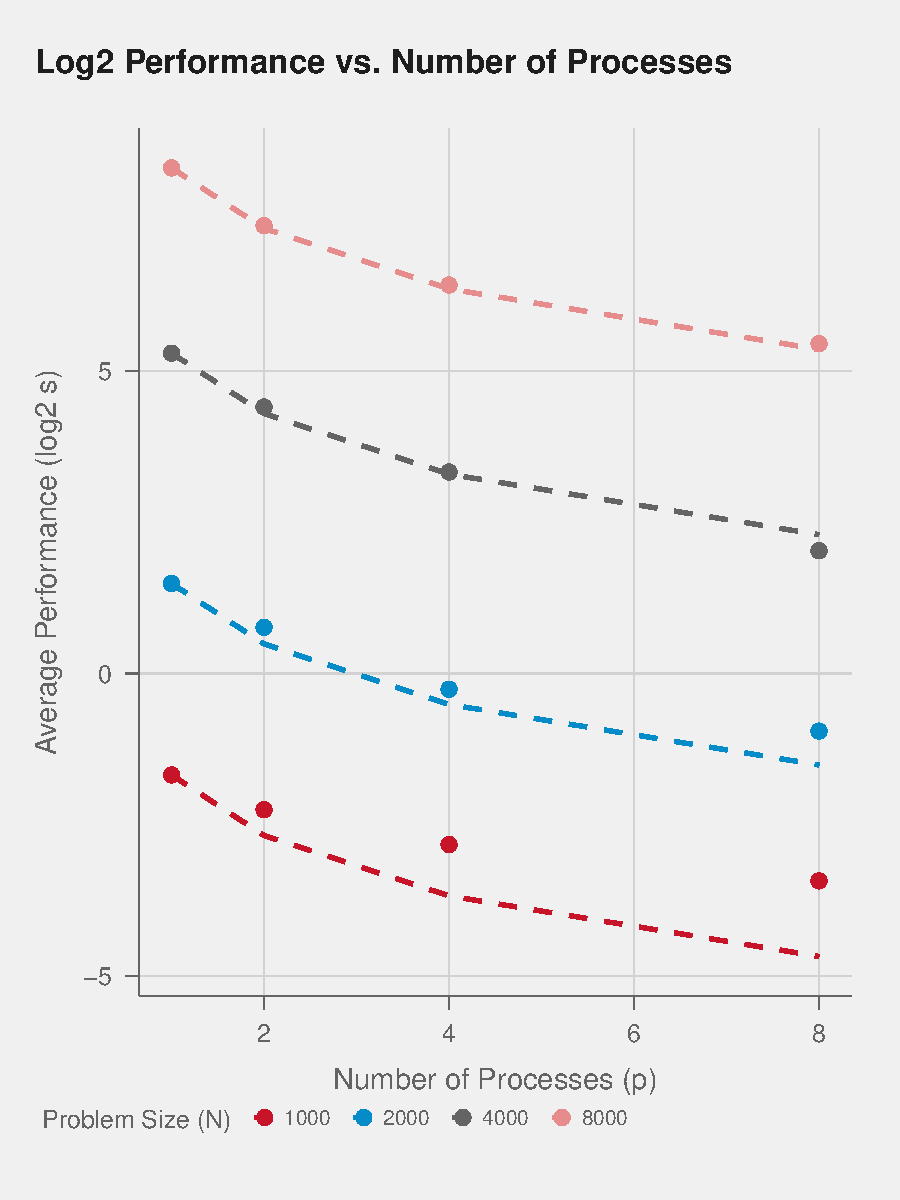
\includegraphics[scale=0.4]{../part2/out/np.pdf} 
   \caption{Blocking Communication: Log2 Performance vs. Number of Processes}
\end{figure}
\noindent The dashed line represents a doubling in performance (halving the runtime) 
as the number of processes doubles relative to the serial runtime. We see that 
for increasing $N$, we achieve closer to the desired throughput via scaling. 
For $N = 1000$, increasing the number of prcesses increases performance but at a 
smaller magnitude relative to larger $N$. It is likely that the overhead in 
communication here is to blame. As $N$ increases, doubling the process count 
just about doubles performance. It seems as though the computational load is 
heavy enough that the communication overhead becomes a smaller fraction of 
the total runtime, allowing for better scalability. That is, the serial portion of a task 
(in this case, the communication overhead) becomes negligible as the problem size increases.

\subsection*{Task 6: Non Blocking Collectives}
Next, we simply replace our blocking collectives with non blocking collectives. 
The algorithm and ring passing stayed entirely the same. What changes was:
\begin{itemize}
    \item \texttt{MPI\_Irecv} and \texttt{MPI\_Isend} instead of \texttt{MPI\_Recv} and \texttt{MPI\_Send}, respectively.
    \item \texttt{MPI\_Iscatter} and \texttt{MPI\_Igather} instead of \texttt{MPI\_Scatter} and \texttt{MPI\_Gather}, respectively.
    \item Adding \texttt{MPI\_Waitall} and \texttt{MPI\_Wait} as necessary, e.g., to ensure the blocks have all been scattered.
\end{itemize}
The performance is seen in Table 2 and Figure 2.
\begin{table}[H]
    \centering
    \caption{Non Blocking Collectives - Average Performance (s)}
    \fontsize{12}{14}\selectfont
    \begin{tabular}[t]{rrrrr}
    \toprule
    p/N & 1000 & 2000 & 4000 & 8000\\
    \midrule
    1 & 0.320 & 3.315 & 40.153 & 328.265\\
    2 & 0.207 & 1.689 & 20.964 & 168.317\\
    4 & 0.126 & 0.816 & 9.993 & 85.030\\
    8 & 0.081 & 0.483 & 3.772 & 43.284\\
    \bottomrule
    \end{tabular}
    \caption*{Comparing MPI non blocking collectives to serial performance as process count increases.}
\end{table}
\begin{figure}[H]
   \centering
   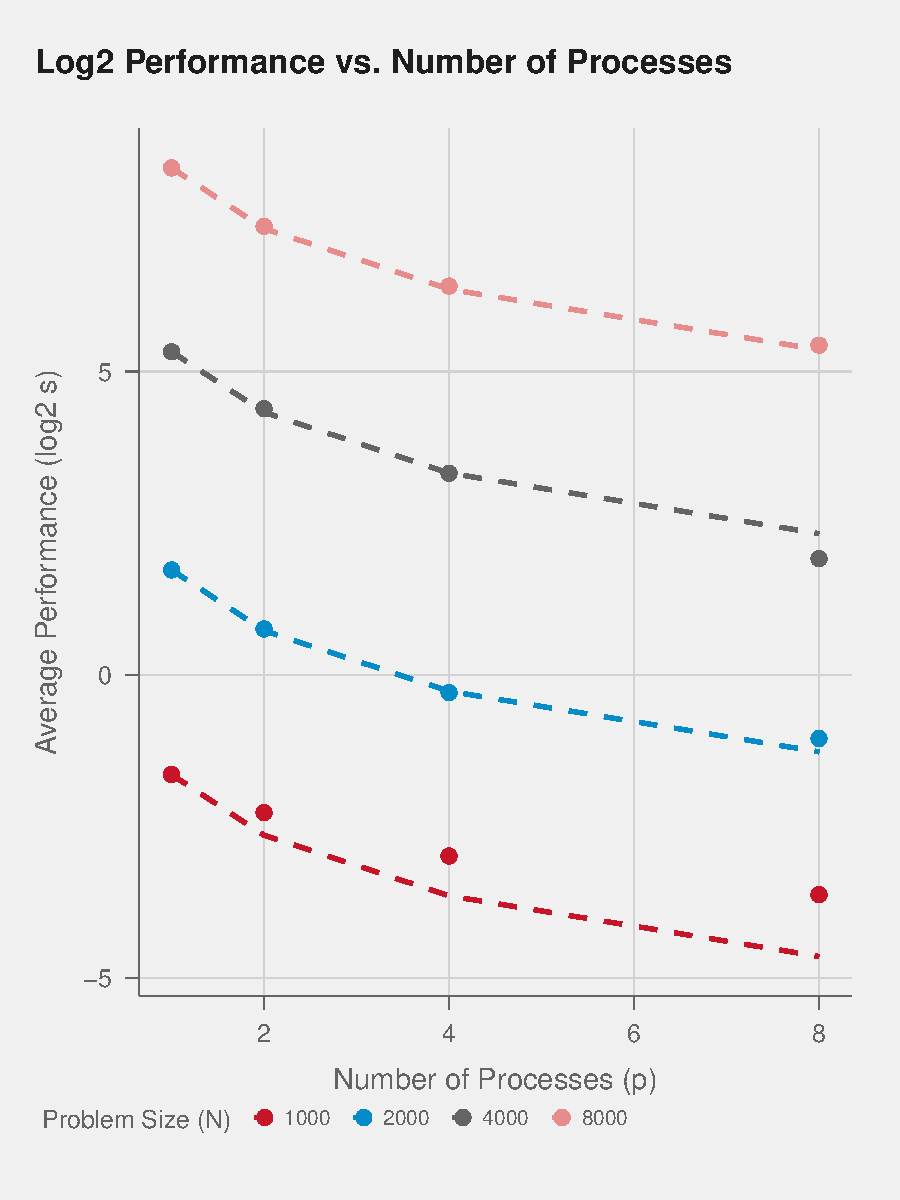
\includegraphics[scale=0.4]{../part2/out/np-6.pdf} 
   \caption{Non Blocking Communication: Log2 Performance vs. Number of Processes}
\end{figure}
\noindent The performance assessment here is precisely that of the blocking collectives. Since 
very little was changed in terms of computation and communication, we expect performance 
to be about similar, as observed.

\subsection*{Task 7: Overlapping Computation and Communication}
Next, we aim to overlap communication and computation. The following items were considered:
\begin{enumerate}
    \item Load Balancing: ideally, the work is evenly distributed among all 
    processes. If some processes finish their work too early, they will be idle while 
    waiting for the others to finish. This is not ideal.
    \item Communication Minimization: We should communicate as little as needed for complete computation.
    \item Overlap: since the \texttt{gemm} function for multiplication does not modify the \texttt{blockB} buffer, 
    we can overlap the send + receive and computation.
\end{enumerate}
The following is the updated ring-loop algorithm:
\begin{lstlisting}
    for (int step = 0; step < size; step++)
    {
        MPI_Irecv(tempB, size_BLOCKxN, MPI_DOUBLE, prev_rank, 0, MPI_COMM_WORLD, &ring_pass_requests[0]);
        MPI_Isend(blockB, size_BLOCKxN, MPI_DOUBLE, next_rank, 0, MPI_COMM_WORLD, &ring_pass_requests[1]);

        gemm(block_size, N, blockA, blockB, blockC, ((rank - step + size) % size) * block_size);

        MPI_Wait(&ring_pass_requests[0], MPI_STATUS_IGNORE);

        double *swap = blockB;
        blockB = tempB;
        tempB = swap;

        MPI_Wait(&ring_pass_requests[1], MPI_STATUS_IGNORE);
    }
\end{lstlisting}
Table 3 and Figure 3 show the performance of these changes:
\begin{table}[H]
    \centering
    \caption{Non Blocking Collectives - Average Performance (s)}
    \fontsize{12}{14}\selectfont
    \begin{tabular}[t]{rrrrr}
    \toprule
    np & 1000 & 2000 & 4000 & 8000\\
    \midrule
    1 & 0.320 & 3.315 & 40.153 & 328.265\\
    2 & 0.206 & 1.647 & 21.035 & 168.214\\
    4 & 0.135 & 0.816 & 9.970 & 85.009\\
    8 & 0.076 & 0.481 & 4.034 & 43.118\\
    \bottomrule
    \end{tabular}
\end{table}
\begin{figure}[H]
    \centering
    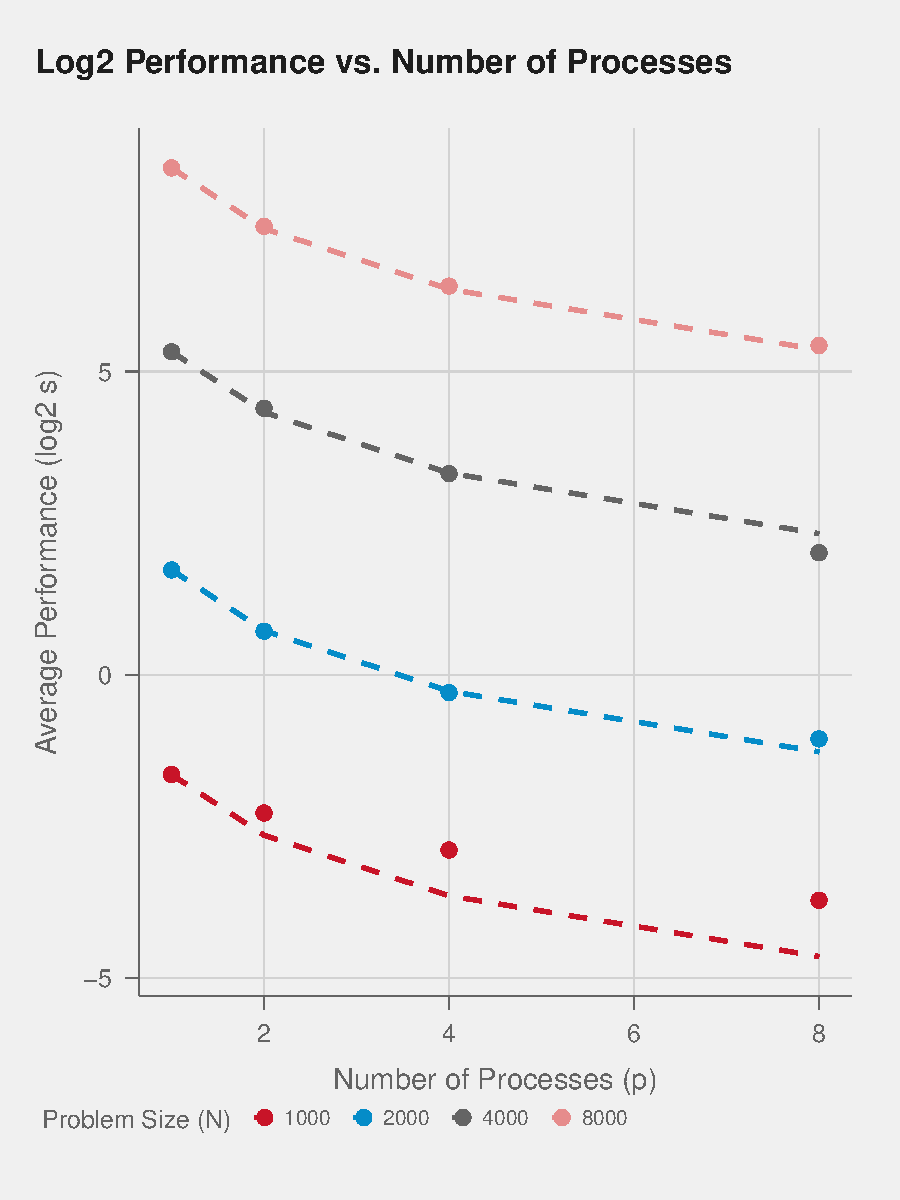
\includegraphics[scale=0.6]{../part2/out/np-7.pdf} 
    \caption{Non Blocking Communication Optimized: Log2 Performance vs. Number of Processes}
 \end{figure}
\noindent We observe roughly the same performance as in task 6. Since each multiply takes the same 
time we are well load balanced and there is minimal idle time by any one process. Moreover, 
we do not overly communicate and we overlap the communication with computation as described. 
Since the communication is such a small amount of the total processing time, we do not expect 
much improvement in performance for this load balanced problem (since any optimizations 
would really come from the multiplication being optimized).

\subsection*{Task 8: Dealing with Non Uniform Buffer Sizes}
Lastly, we modify the blocking collectives code to handle the case where $N$ 
is not divisible by $p$. The following had to be considered (in continuation from task 5):
\begin{itemize}
    \item $N/p$ will have a remainder, i.e., $N \% p$. This remainder 
    will be less than the total number of processes and so all ranks less than 
    the remainder will get $\mathsf{floor}(N/p) + 1$ rows (or columns) and the 
    rest of the ranks get $\mathsf{floor}(N/p)$ rows (or columns).
    \begin{itemize}
        \item Now, every \texttt{blockA}, \texttt{blockB}, or \texttt{blockC} has 
        array size $(\texttt{floor}(N/p) + 1) \times N$ or $\texttt{floor}(N/p) \times N$. 
    \end{itemize}
    \item For the initial assignments, $\texttt{MPI\_Scatterv}$ is used with the appropriately passed 
    in displacements array to distribute the blocks.
    \begin{itemize}
        \item Each process still gets a permanant allocation of \texttt{blockA} and \texttt{blockC} and 
        starts with an initial assignment of \texttt{blockB}.
        \item Each process allocates a size for \texttt{blockB} and \texttt{tempB} that is the largest possible size.
        In doing so, the differently sized buffers can be passed around without having to reallocate memory.
        \item At each time step on a process, a multiply might be between:
        \begin{enumerate}
            \item An $(\texttt{floor}(N/p) + 1) \times N$ \texttt{blockA} and an $N \times (\texttt{floor}(N/p) + 1)$ \texttt{blockB}.
            \item An $(\texttt{floor}(N/p) + 1) \times N$ \texttt{blockA} and an $N \times \texttt{floor}(N/p)$ \texttt{blockB}.
            \item An $\texttt{floor}(N/p) \times N$ \texttt{blockA} and an $N \times (\texttt{floor}(N/p) + 1)$ \texttt{blockB}.
            \item An $\texttt{floor}(N/p) \times N$ \texttt{blockA} and an $N \times \texttt{floor}(N/p)$ \texttt{blockB}.
        \end{enumerate}
    \end{itemize}
    \item At step $i$ in the ring swap, process $p$ is working on the \texttt{blockB} initially allocated to rank \texttt{(rank - i + p) \% p}.
    The size of each ranks initial allocation is kept track of to appropriately index the \texttt{blockB} array for multiplication 
    (since it is allocated to the maximum possible size it may have data in it we do not want). The result of the multiply is placed in the correct sub-block of \texttt{blockC}.

\end{itemize}
The resulting code is an algorithm that produces the following performance and 
$F$-norm on an $N = 7633$, $p = 7$ program run on 4 nodes (the manager alone 
on one node and the other 3 nodes having two processes):\footnote{
    The distribution of the processes is done with a hostfile and was done via 
    a back and forth consultation with ChatGPT. The resource allocation with the 
    hostfile is NOT original work. The script is in \texttt{build-run-task8.sh}.
}
\begin{table}[H]
    \centering
    \caption{Non Uniform Size Allocation with Blocking Collectives}
    \fontsize{12}{14}\selectfont
    \begin{tabular}[t]{rrrr}
    \toprule
    p & N & time & F-norm\\
    \midrule
    7 & 7633 & 41.70652 & 1.535e-09\\
    \bottomrule
    \end{tabular}
\end{table}
\noindent Here is a sample of reported bindings
\begin{verbatim}
Task 8
[r918u05n01.grace.ycrc.yale.edu:1515798] MCW rank 0 bound to socket 0[core 0[hwt 0]]: [B][.]
[r918u05n03.grace.ycrc.yale.edu:636934] MCW rank 3 bound to socket 0[core 0[hwt 0]]: [B][.]
[r918u05n03.grace.ycrc.yale.edu:636934] MCW rank 4 bound to socket 1[core 1[hwt 0]]: [.][B]
[r918u05n02.grace.ycrc.yale.edu:380664] MCW rank 1 bound to socket 0[core 0[hwt 0]]: [B][.]
[r918u05n02.grace.ycrc.yale.edu:380664] MCW rank 2 bound to socket 1[core 1[hwt 0]]: [.][B]
[r918u05n04.grace.ycrc.yale.edu:1996065] MCW rank 5 bound to socket 0[core 0[hwt 0]]: [B][.]
[r918u05n04.grace.ycrc.yale.edu:1996065] MCW rank 6 bound to socket 1[core 1[hwt 0]]: [.][B]
\end{verbatim}
We see that the algorithm runs in a reasonably expected time and produces near 
0 $F$-norm.

\section{Conclusion}
In conclusion, we have demonstrated the effectiveness of OpenMPI for parallel matrix multiplication.
Key insights include the significance of balancing computational load and communication overhead, 
particularly in larger matrix computations. The analysis revealed that while increasing the 
number of processors generally enhances performance, the impact varies with the problem size, 
indicating the necessity for a parallelization strategy that is based on the problems
specific computational requirements. 

\end{document}

